\chapter{Stabilità nei sistemi dinamici}


\section{Sistema dinamico e punti di equilibrio}

Un sistema dinamico 
è composta da uno stato \(x \in \mathbb{R}^{n}\)
e da una legge di evoluzione

\begin{equation}
  \dot{x}(t) = f(x(t), u(t), t)
  \label{sistema-dinamico-generale}
\end{equation}

\begin{definizione}
Un sistema è detto \textbf{tempo invariante} se la
  sua evoluzione non dipende esplicitamente dal tempo \(t\), cioè:
  \[\dot{x}(t) = f(x(t), u(t))\]
\end{definizione}


\begin{definizione}
Un sistema è detto \textbf{autonomo} se la sua evoluzione non dipende esplicitamente
  dall'ingresso \(u(t)\), cioè:
  \[\dot{x}(t) = f(x(t),t)\]
\end{definizione}

Se il sistema è sia autonomo che tempo invariante
allora si ha:
\[\dot{x}(t) = f(x(t))\]




\begin{definizione}
Dato un sistema dinamico \textbf{tempo invariante} nella forma:
\[\dot{x}(t) = f(x(t), u(t))\]
un punto di equilibrio \((\bar{x}, \bar{u})\) è una coppia 
stato-ingresso tale che:
\[\dot{x} = f(\bar{x}, \bar{u}) = 0\]


\end{definizione}



\section{Stabilità e Convergenza}



\begin{definizione}

Un sistema dinamico 
tempo invariante è detto stabile se 

\begin{equation}
  \forall \varepsilon > 0, 
  \exists \delta > 0 : x_{0} 
  \in B_{\delta}(\bar{x})
  \Rightarrow |x_{x_{0}}(t) - \bar{x}| \le \varepsilon, \forall t \geq 0
  \label{stabilità}
\end{equation}Dove con \(x_{x_{0}}(t)\) si intende 
la traiettoria del sistema 
che parte da \(x_{0}\).
\end{definizione}



Ora dimostriamo che \(\delta \le 
\varepsilon ,
\forall \varepsilon > 0\).
\begin{proof}
  
Supponiamo per assurdo che 
esista un \(\varepsilon >0 \)
per cui si ha  
che la \(\delta\)
per cui è rispettata la 
definizione di stabilità sia
tale che
\(\delta > \varepsilon\).
Allora si ha che per
le 
\(x_{0} \in B_{\delta}(\bar{x}) \backslash
B_{\varepsilon}(\bar{x})\)
vale:
\[|x_{x_{0}}(0) - \bar{x}| 
= \left|x_{0} -\bar{x}\right|> \varepsilon\]
Ma questo è assurdo perché
\(x_{0} 
\in B_{\delta}(\bar{x})\)
dunque rispetta la definizione 
di stabilità per cui
si dovrebbe avere :
\[|x_{x_{0}}(0) - \bar{x}| 
= \left|x_{0} - \bar{x}\right|
\le \varepsilon
\]
Dunque siamo arrivati ad un assurdo.

\end{proof}



\begin{definizione}
  Dato un sistema dinamico un punto di equilibrio
  \(\bar{x}\) è detto \textbf{convergente} se esiste un 
  \(\delta >0\) tale che per ogni condizione iniziale
  \(x_{0} \in B_{\delta}(\bar{x})\) si ha che:
  \[\lim_{t \to \infty} \left|\left|x(t) - \bar{x}\right|\right| = 0\]

\end{definizione}

\begin{definizione}
  Un punto di equilibrio \(\bar{x}\) è detto 
  \textbf{isolato} se esiste un intorno di \(\bar{x}\)
  che non contiene altri punti di equilibrio.
\end{definizione}


% ...existing code...
\begin{figure}[htbp]
  \centering
  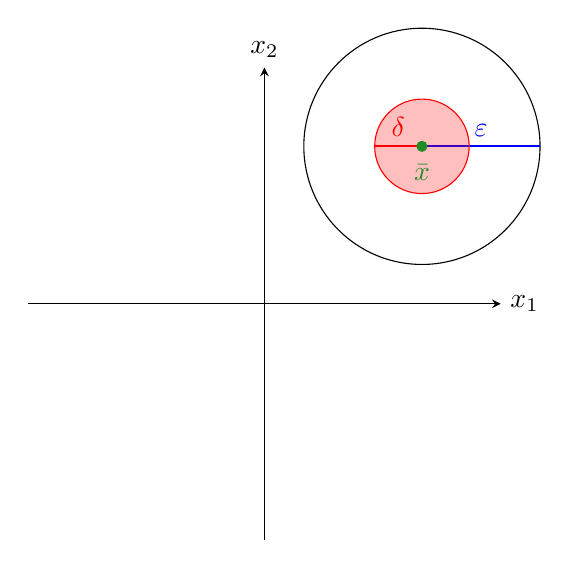
\begin{tikzpicture}[scale=1, >=stealth]
    % assi con sole etichette x1 e x2
    \draw[->] (-3,0) -- (3,0) node[right] {$x_1$};
    \draw[->] (0,-3) -- (0,3) node[above] {$x_2$};


    % cerchio grande e raggio epsilon
    \draw (2,2) circle (1.5);
    \draw[thick, blue] (2,2) -- ++(1.5,0) node[midway, above] {$\varepsilon$};

    % cerchio piu' piccolo rosso trasparente e raggio delta (più corto)
    \filldraw[fill=red, fill opacity=0.25, draw=red] (2,2) circle (0.6);
    \draw[thick, red] (2,2) -- ++(-0.6,-0) node[midway, above] {$\delta$};

    \filldraw[ForestGreen] (2,2) circle (1.8pt) node[below=3pt] {$\bar{x}$};

  \end{tikzpicture}
  \caption{In \textcolor{ForestGreen}{verde} si ha il 
  punto di equilibrio \textcolor{ForestGreen}{\(\bar{x}\)}. 
  In rosso si ha l'insieme delle condizioni iniziali per cui le traiettorie rimangono
  confinate  all'interno del cerchio di raggio \(\varepsilon\).}
  \label{fig:assi-x1-x2}
\end{figure}
% ...existing code...
\section{Stabilità nei sistemi lineari}

Consideriamo un sistema lineare
tempo invariante:
\[\dot{x}(t) = Ax(t) + Bu(t)\]
Dove \(A \in \mathbb{R}^{n \times n}\) e 
\(B \in \mathbb{R}^{n \times m}\).
Per trovare i punti di equilibrio dobbiamo imporre:
\[\dot{x}(t) = 0 \Longleftrightarrow Ax(t) + Bu(t) = 0\]
Dunque i punti di equilibrio 
sono le coppie \((\bar{x}, \bar{u})\) che soddisfano:
\[ 
A\bar{x} + B\bar{u} = 0
\]
Notiamo subito che il punto \((\bar{x}, \bar{u}) = (0,0)\)
 è sicuro un punto di equilibrio.
Mentre gli altri punti si trovano risolvendo il sistema lineare
omogeneo considerando \(\bar{x}\) e \(\bar{u}\) come incognite.
Se invece di considerare le coppie \((\bar{x}, \bar{u})\) di equilibrio
consideriamo solo gli stati di equilibrio \(\bar{x}\) con un 
fissato \(\bar{u}\), allora l'unica incognita è \(\bar{x}\) 
mentre \(B \bar{u}\) è un termine noto.
In questo caso il sistema lineare da risolvere è:
\[A \bar{x} = - B \bar{u}\]
Questo sistema al variare di \(\bar{u}\) 
(che funge da parametro) ammette soluzioni differenti,
però la matrice \(A\) ci dice quante sono queste soluzioni.
Se \(A\) è invertibile (ovvero \(\det(A) \neq 0\))
allora esiste un'unica soluzione per ogni \(\bar{u}\):
\[\bar{x} = -A^{-1}B \bar{u}\]
Se invece \(A\) non è invertibile (ovvero \(\det(A) = 0\))
allora il sistema può ammettere infinite soluzioni oppure nessuna soluzione
(ricordiamo che il sistema si risolve
al variare del parametro \(\bar{u}\)).

\section{Sistema nel dominio di Laplace}
Consideriamo il sistema lineare tempo invariante:
\[\dot{x}(t) = Ax(t) + Bu(t)\]
Applichiamo la trasformata di Laplace ambo i membri otteniamo:
\[sX(s) - x(0) = AX(s) + BU(s)\]
Portando \(x(0)\) a destra e portando \(AX(s)\) a sinistra otteniamo:
\[sX(s) - AX(s) = BU(s) + x(0)\]
Ricordando che \(sX(s) = s I X(s)\) e mettendo in evidenza \(X(s)\) otteniamo:
\[(sI - A)X(s) = BU(s) + x(0)\]
Ora premoltiplichiamo ambo i membri per
\((sI - A)^{-1}\) otteniamo:
\[X(s) = \textcolor{red}{(sI - A)^{-1}BU(s)} + \textcolor{blue}{(sI - A)^{-1}x(0)}\]
Dove in \textcolor{red}{rosso} abbiamo la parte dovuta all'ingresso
che prende il nome di \textcolor{red}{evoluzione forzata}  dello stato, 
mentre in \textcolor{blue}{blu}
abbiamo la parte dovuta alla  \textcolor{blue}{evoluzione libera}
dello stato (che ricordiamo essere nulla se \(x(0) = 0\)).
Andando a fare la stessa cosa per l'equazione di uscita:
\[y(t) = Cx(t) + Du(t)\]
Applichiamo la trasformata di Laplace otteniamo:
\[Y(s) = CX(s) + DU(s)\]
Sostituendo \(X(s)\) otteniamo:
\[Y(s) = C\left[(sI - A)^{-1}BU(s) + (sI - A)^{-1}x(0)\right] + DU(s)\]
Dove riusciamo un'altra volta a distinguere una parte
in \textcolor{red}{evoluzione forzata} ed un una in \textcolor{blue}{
evoluzione libera}:
\[Y(s) =\textcolor{red}{C \left[\left(sI - A\right)^{-1} + D\right]BU(s)} +
\textcolor{blue}{ 
\left(sI - A\right)^{-1}x(0)} \]


\section{Teorema di Lyapunov}

Ora ci interessa introdurre un metodo per studiare la stabilità
dei sistemi dinamici che prende il nome di \textbf{approccio di Lyapunov},
che ci permette di studiare la stabilità dei sistemi andandoci a 
trovare delle specifiche funzioni 
scalari \(V(x) : 
\mathbb{R}^n \to \mathbb{R}\) dette \textbf{funzioni di Lyapunov}.
Per prima cosa ricordiamo che una funzione \(V(x) : \mathbb{R}^{n} 
\to \mathbb{R}\) e un suo punto di equilibrio 
possono essere classificati come:
\begin{itemize}
  \item \textbf{definita positiva} 
  in \(\bar{x}\) se \(V(\bar{x}) = 0\) ed esiste un \(\delta > 0\)
  tale che \(V(x) > 0\) (notiamo il maggiore stretto) per ogni \(x \in B_{\delta}(\bar{x})\)
  \item \textbf{semidefinita positiva} 
  in \(\bar{x}\) se \(V(\bar{x}) = 0\) ed esiste un \(\delta > 0\)
  tale che \(V(x) \ge 0\) per ogni \(x \in B_{\delta}(\bar{x})\)
  \item \textbf{definita negativa} 
  in \(\bar{x}\) se \(V(\bar{x}) = 0\) ed esiste un \(\delta > 0\)
  tale che \(V(x) < 0\) per ogni \(x \in B_{\delta}(\bar{x})\)
  \item \textbf{semidefinita negativa} 
  in \(\bar{x}\) se \(V(\bar{x}) = 0\) ed esiste un \(\delta > 0\)
  tale che \(V(x) \le 0\) per ogni \(x \in B_{\delta}(\bar{x})\)
\end{itemize}
Queste proprietà diventano \textbf{globali}
quando sono vere per ogni \(\bar{x} \in \mathbb{R}^{n}\).
La potenza del metodo che stiamo per introdurre
sta nel fatto che è valida anche per sistemi non lineari,
nel momento in cui aggiungeremo l'ipotesi di linearità andremo 
ad ottenere anche altri risultati.

\begin{teorema}
Teorema di Lyapunov.  Consideriamo il sistema dinamico:
\[\dot{x}(t) = f(x(t))\]
Consideriamo il punto di equilibrio \(\bar{x}\) per \(f\).
Se \(f\) è definita, è continua ed anche la sua derivata è continua
in un intorno \(D\) di \(\bar{x}\),
cioè \(f \in C^{1}(D)\) (\(f\) 
è un vettore di funzioni quindi quando diciamo che è 
continua intendiamo che ogni sua componente lo è).
Se esiste una funzione \(V(x) : \mathbb{R}^{n} \to \mathbb{R}\), 
continua e derivabile in \(D\), tale che:
\begin{itemize}
  \item \(V(x)\) è definita positiva in \(\bar{x}\), cioè:
  \[\begin{cases}
    V(\bar{x}) = 0 \\
    \exists \delta : V(x) > 0, \quad \forall x \in B_{\delta}(\bar{x}) \backslash \{\bar{x}\}
  \end{cases}\]
  \item \(\dot{V}(x)\) è semidefinita negativa in \(\bar{x}\), cioè:
  \[\begin{cases}
    V_{\bar{x}} = 0 \\
    \exists \delta : \dot{V}(x) = \nabla V(x) \cdot 
    \displaystyle 
    \frac{dx}{dt} = \nabla V(x(t)) f(x(t)) \le 0, \quad \forall x \in B_{\delta}(\bar{x})
  \end{cases}\]
\end{itemize}
Allora si ha che il punto di equilibrio \(\bar{x}\) è stabile.
\end{teorema}

\begin{proof}
Noi vogliamo dimostrare che \(\bar{x}\) è un punto di equilibrio stabile,
cioè che per ogni \(\varepsilon > 0\) esiste un \(\delta > 0\)
tale che se \(x_{0} \in B_{\delta}(\bar{x})\) allora
la traiettoria \(x(t)\) che parte da \(x_{0}\)
rimane confinata in \(B_{\varepsilon}(\bar{x})\).
Dunque partiamo con il fissare un generico \(\varepsilon > 0\).
Consideriamo l'insieme \(S = \left\{x \in \mathbb{R}^{n} : \left|\left|x\right|\right| =
\varepsilon \right\} \).

Deve esistere una curva di livello di \(V(x)\) di valore \(\bar{V}\)
completamente contenuta in \(B_{\varepsilon}(\bar{x})\), come 
in Figura \ref{fig:lyapunov-curve-level}. Ora chiamiamo \(\delta\)
la distanza minima tra \(\bar{x}\) e la curva di livello di valore \(\bar{V}\).
Ora consideriamo una \(x(t)\)
che parte da un punto \(x_{0} \in B_{\delta}(\bar{x})\) 
\((x(0) = x_{0})\). A noi interessa dimostrare che \(\bar{x}\) è
stabile, cioè che \(\forall x_0 \in B_{\delta}(\bar{x})\)
la traiettoria \(x(t)\) rimane confinata nella curva di livello di valore \(\bar{V}
\forall t \ge 0\),
questo implica che \(x(t)\) rimane confinata anche all'interno di 
\(B_{\varepsilon}(\bar{x})\) ( questo perché \(\bar{V}\) 
è completamente contenuta all'interno di \(B_{\varepsilon}(\bar{x})\)).
Dunque per dimostrare la stabilità dobbiamo dimostrare che
\(x(t)\) non può uscire dalla curva di livello
(ricoridamo che \(V(x)\) è funzione di \(x\) quindi una curva di livello
è una curva nello spazio di stato) di valore \(\bar{V}\). Poichè \(\dot{V}(x) \le 0\)
allora \(V(x(t))\) è una funzione decrescente nel tempo,

\end{proof}


Se \( f \in C^{1}(D) \) allora è anche sicuramente
 localmente Lipschitziana
in  \(D\) (poichè se una funzione è \(C^{1}\) allora 
il suo gradiente è limitato) cioè:
\[\exists L >0  : \|f(x) - f(y)\| \le L \|x - y\|, \quad \forall x,y \in I\] 